 \documentclass[h]{article}
\usepackage[margin=0.5in]{geometry}
\usepackage{amsfonts} 
\usepackage{textcomp}
 
\usepackage{graphicx}
\usepackage{caption}
\usepackage{subcaption}
\usepackage{float} 
\usepackage{flafter}
\graphicspath{ {./plots/} }
\usepackage{adjustbox}


\newcommand{\cent}{\textcent \hspace{4pt}}
\title{CS 7641 Machine Learning \\ Assignment 2}
\date{Due Sunday March 11th, 2018 11:59pm}
\author{Philip Bale \\ pbale3}

\begin{document}

\maketitle

\section*{Part 1: Neural Network Optimization}
\subsection*{ Introduction}  
Part 1 of the assignment surrounds using randomized optimization to find the 
best possible weights for a specific neural network.  In assignment 1, backpropogation 
was used to find optimal parameters for a neural network.  This neural network 
took in various input features for US permanent visa applicants and then 
attempted to predict the outcome of an application.  After various tests, I found the optimal parameters of: 6-node input layer, one hidden layer with 100 nodes, 
one output node, and about 500 iterations.
\\ \\
For assignment 2, three other optimization strategies are employed to find 
optimal weights: randomized hill climbing, simulated annealing, and genetic 
algorithms.  The details of each are discussed in-depth further in this section 
and an analysis is performed for each strategy to evaluate its results.  It is 
important to note that this network does tend to converge quite quickly due to  
its size and consistant distribution.
\\ \\ 
I primarily chose this problem domain because, as someone who has worked 
with a large number of first-generation visa holders and immigrants, I am 
extremely interested in building tools to help others to achieve the same.  At the end of the day, the goal is it to try to determine the application result 
before time, money, and other resources are spent.
\\ \\

\subsection*{1) Backpropogation (Assignment 1)}  
\subsubsection*{Overview}
The first weight-finding algorithm used was backpropogation.  Backpropogation works by essentially calculating 
the error at the end of a network, and then working backwards to minimize that error over various iterations. 
 An error (or loss) function is effectively minimized over time using this backpropogation technique.   As discussed in assignment 1, the permanent 
 visa is rather large and robust.  It is quickly learnable by various different 
 learners and in such backpropogation found significant success.
 
 \begin{figure}[H]
  \minipage{0.49\textwidth}
      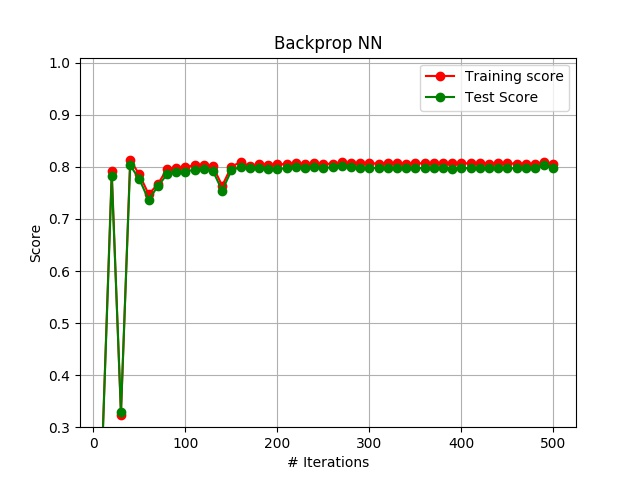
\includegraphics[width=1\textwidth,keepaspectratio]{backprop_nn_1.jpg} 
      \caption*{Backprop NN Success Rate vs. Iterations} 
   \endminipage\hfill
   \minipage{0.49\textwidth}
      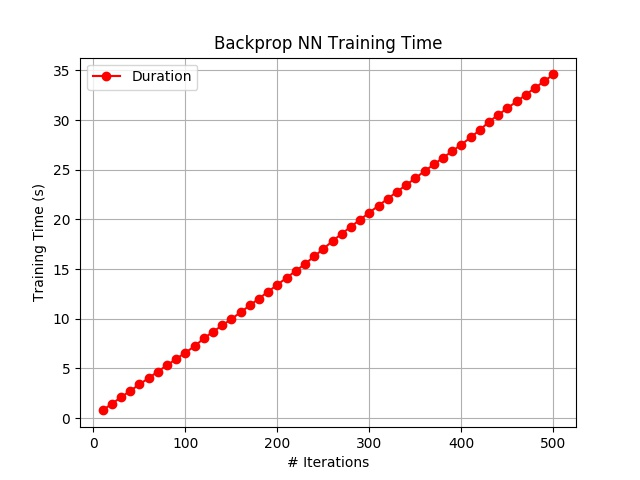
\includegraphics[width=1\textwidth,keepaspectratio]{backprop_nn_time_1.jpg} 
      \caption*{Backprop NN Training Time} 
   \endminipage\hfill
\end{figure}

Right around 50 iterations, the network begins to converge at around an 80\% 
successs rate.  Seeing as the training and test score track either rather 
closely, it is apparent that the dataset is rather robust and consistent.  One 
thing to note is that the training time scales linearly with the number of 
iterations--which makes sense since the same amount of calculations with similar 
complexity are performed on each iteration of backpropogation.  

\subsection*{2) Randomized Hill Climbiing}  
\subsubsection*{Overview}
The second weight-finding algorithm used was randomized hill climbing.  
Randomized hill climbing works by taking a random starting point and then 
incrementally attempting to improve on that point.  In the context of a neural 
network trying to find weights,  randomized hill climbing selects random weights 
and then moves in a direction so as to try to find a better result for that 
weight--akin to trying to move up an optimization 'success hill'.
\\ \\ 
One thing to 
note is that we are using randomized hill climbing, not random restart hill 
climbing.  In such, the algorithm is prone to getting caught in local optimizations, or local maximums. 


 \begin{figure}[H]
  \minipage{0.49\textwidth}
      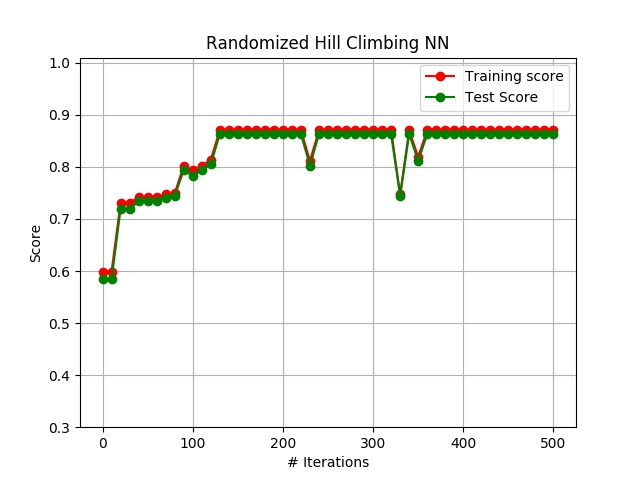
\includegraphics[width=1\textwidth,keepaspectratio]{randomized_hill_climbing_nn.jpg} 
      \caption*{Randomized Hill Climbing NN Success Rate vs. Iterations} 
   \endminipage\hfill
   \minipage{0.49\textwidth}
      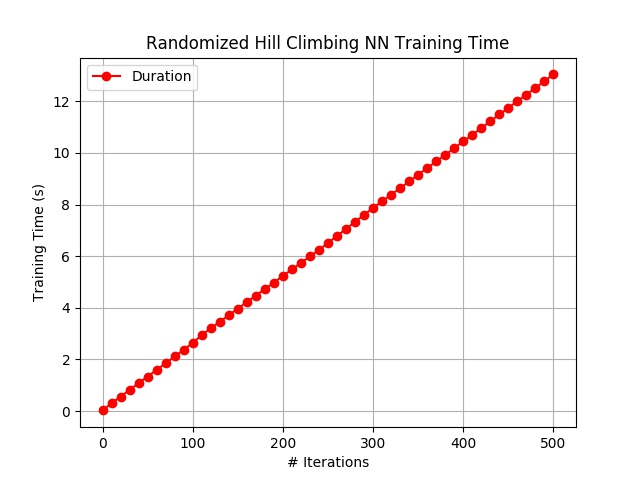
\includegraphics[width=1\textwidth,keepaspectratio]{randomized_hill_climbing_nn_time.jpg} 
      \caption*{Randomized Hill Climging NN Training Time} 
   \endminipage\hfill
\end{figure}

High accuracy results are achieved right around 125 iterations+.  
While this is subject to randomness, by looking at the results it is shown to 
become rather consistant.  By looking at the score results, one can see various 
instances of the randomized hill climbing getting caught in local optimas and 
being unable to escape.  Such is the case around 220, 320, and 350 iterations.
\\ \\
Similar to backpropogation, training time scales linearly with the number of 
 iterations run. Training time tends to be a bit faster using randomized hill 
 climbing because of a reducation in calculations necessary.  Whereas 
 backpropogation needed to do calcluations to minimize error moving backwards 
 through the network, randomized hill climbing simply needs to move in one 
 direction and determine if the new weights are better.
 
\subsection*{3) Simulated Annealing}  
\subsubsection*{Overview}
The third weight-finding algorithm used was simulated annealing.  Simulated 
annealing works by taking a random solution and then samples nearby 
alternatives.  By comparing the alternatives to the original solution, the 
optimizer decides to either stick with the original solution or move to the new 
one.  Using a temperature and cooling parameter, the algorithm is more open to 
worse solutions at first but gradually moves towards only accepting better 
solutions.
\\ \\
Various coolng parameters were used to try to determine the best simulate 
annealing approach.  Below, success rates by number of iterations are showed for 
simulated annealing approaches with cooling parameters of .15, .35, and .7.  The 
parameter of .15 and .35 take significantly longer to converge to the optimal 
solution than did a higher parameter.  While part of this can be attribute to 
luck (the algorithm could have randomly found itself in an optimal solution earlier 
on)--part of this too is the way the algorithm operates by its parameters.  The 
.7 cooling temperature here proved most effective.

 \begin{figure}[H]
  \minipage{0.49\textwidth}
      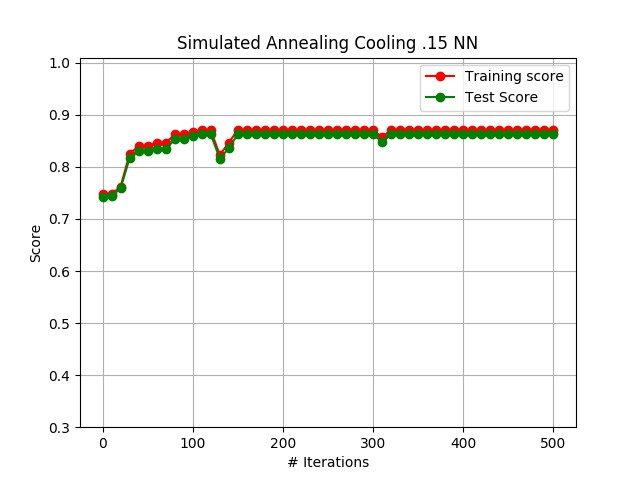
\includegraphics[width=1\textwidth,keepaspectratio]{simulated_annealing_cooling_pt15_nn.jpg} 
      \caption*{Simulated Annealing NN Success Rate vs. Iterations w/ .15 Cooling} 
   \endminipage\hfill
   \minipage{0.49\textwidth}
      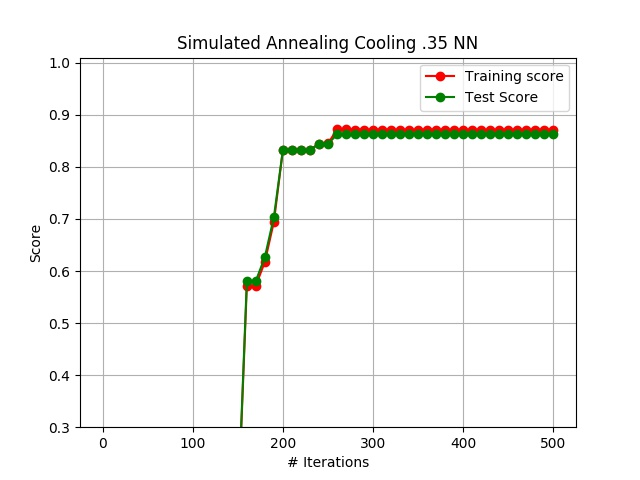
\includegraphics[width=1\textwidth,keepaspectratio]{simulated_annealing_cooling_pt35_nn.jpg} 
      \caption*{Simulated Annealing NN Success Rate vs. Iterations w/ .35 Cooling} 
   \endminipage\hfill
\end{figure}

 \begin{figure}[H]
  \minipage{0.49\textwidth}
      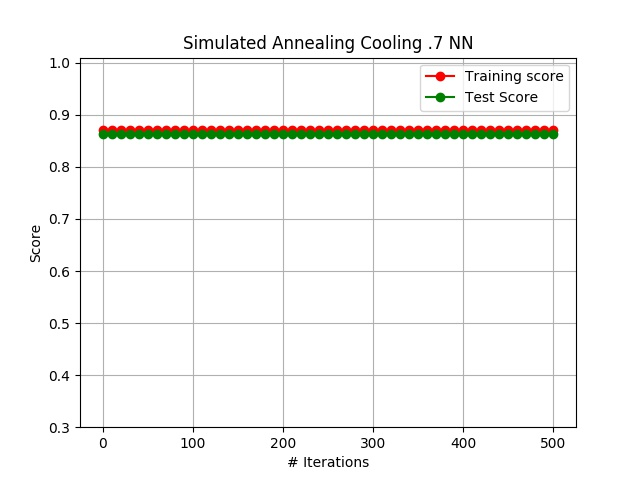
\includegraphics[width=1\textwidth,keepaspectratio]{simulated_annealing_cooling_pt7_nn.jpg} 
      \caption*{Simulated Annealing NN Success Rate vs. Iterations w/ .7 Cooling} 
   \endminipage\hfill
   \minipage{0.49\textwidth}
      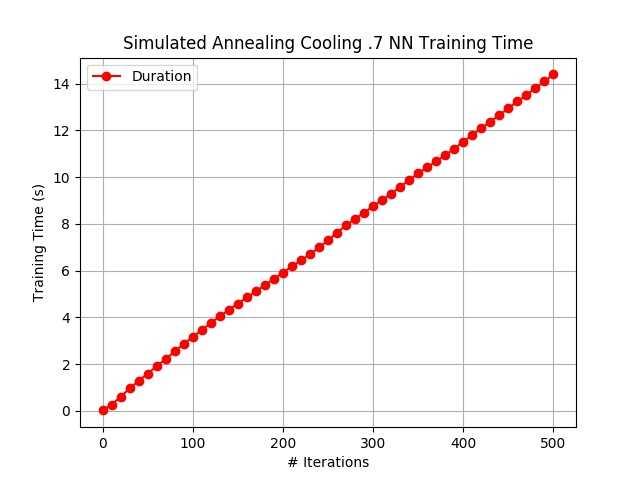
\includegraphics[width=1\textwidth,keepaspectratio]{simulated_annealing_cooling_pt7_nn_time.jpg} 
      \caption*{Simulated Annealing NN Training Time w/ .7 Cooling} 
   \endminipage\hfill
\end{figure}

\subsection*{4) Genetic Algorithms}  
\subsubsection*{Overview}
The fourth weight-finding algorithm used was a genetic algorithm.  Genetic 
algorithms works by starting with an initial solution and then making 
modifications in an attempt to improve the solution.  The modifications 
generally allowed are mutation (changing random parts of the solution), crossover (taking specific sections
 from various solutions and combining them), and selection (selecting certain sections from a solution to use again). 
  In the context of a neural network, we can use genetic algorithms to make 
  modifications to our network's weights.
 \\ \\ 
 In our testing, a population size of 50 was used in order to get a diverse 
 initial sampling of possible solutions.  The number of instances to mate (aka crossover) and to 
 mutate was varied throughout the trials.
 
  \begin{figure}[H]
  \minipage{0.49\textwidth}
      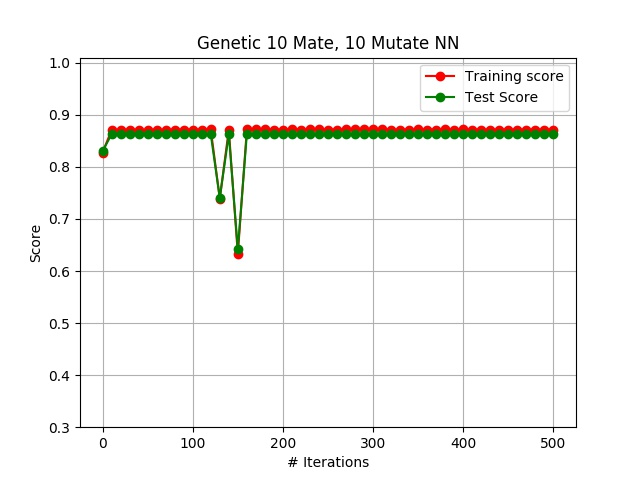
\includegraphics[width=1\textwidth,keepaspectratio]{genetic_10_mate,_10_mutate_nn.jpg} 
      \caption*{Genetic Algorithm Success Rate v. Iterations w/ 10 Mate, 10 Mutate,  50 population} 
   \endminipage\hfill
   \minipage{0.49\textwidth}
      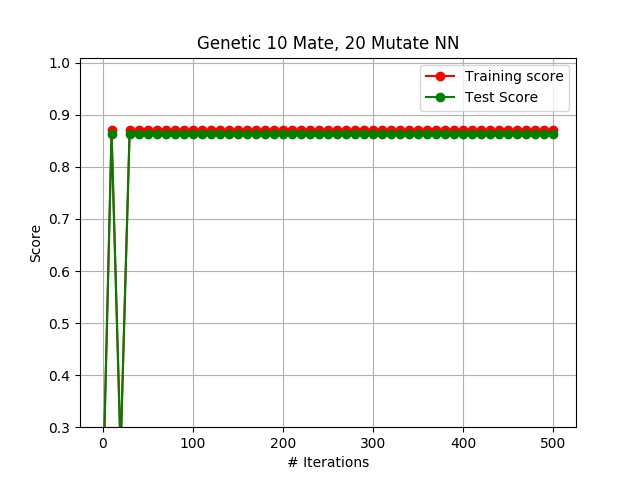
\includegraphics[width=1\textwidth,keepaspectratio]{genetic_10_mate,_20_mutate_nn.jpg} 
      \caption*{Genetic Algorithm Success Rate v. Iterations w/ 10 Mate, 20 Mutate,  50 population} 
   \endminipage\hfill
\end{figure}

 \begin{figure}[H]
  \minipage{0.49\textwidth}
      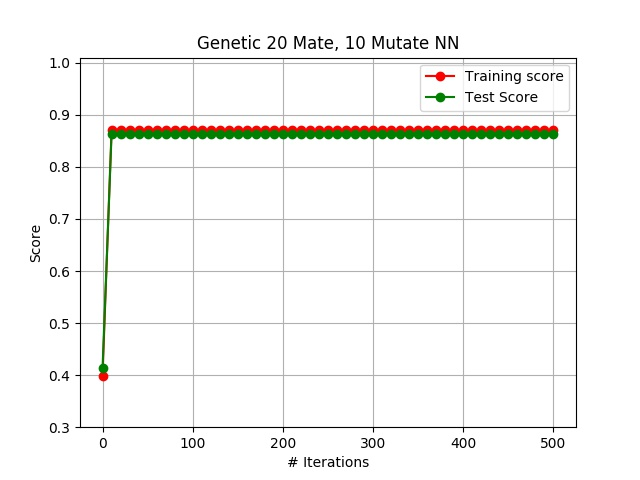
\includegraphics[width=1\textwidth,keepaspectratio]{genetic_20_mate,_10_mutate_nn.jpg} 
      \caption*{Genetic Algorithm Success Rate v. Iterations w/ 20 Mate, 10 Mutate,  50 population} 
   \endminipage\hfill
   \minipage{0.49\textwidth}
      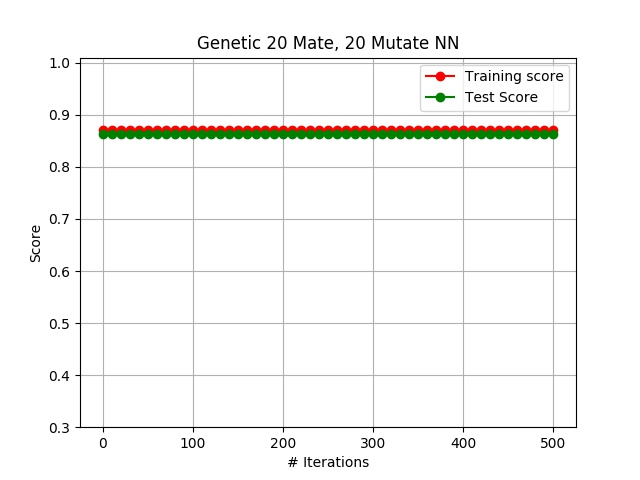
\includegraphics[width=1\textwidth,keepaspectratio]{genetic_20_mate,_20_mutate_nn.jpg} 
      \caption*{Genetic Algorithm Success Rate v. Iterations w/ 20 Mate, 20 Mutate, 50 population} 
   \endminipage\hfill
\end{figure}

Trials were run with the following mate/mutate combinations:  10/10, 10/20, 
/20/10, and 20/20.  All trials were run with a population size of 50.  As can be 
observed from the graphs, both mating and mutating appeared to be highly 
effective in finding the optimal solution.  In fact, the optimal solution 
converged quite quickly--in under 30 iterations for each trial.  This is partly 
due to the fact that the data is easily learnable and does not appear to 
maintain very many trapping local maximums.
\\ \\
Training times scaled roughly linearly with the number of iterations ran.  This 
makese sense because, from a performance perspective, the number of mutation 
calculations from iteration to iteration is more or less the same.

 \begin{figure}[H]
  \minipage{0.49\textwidth}
      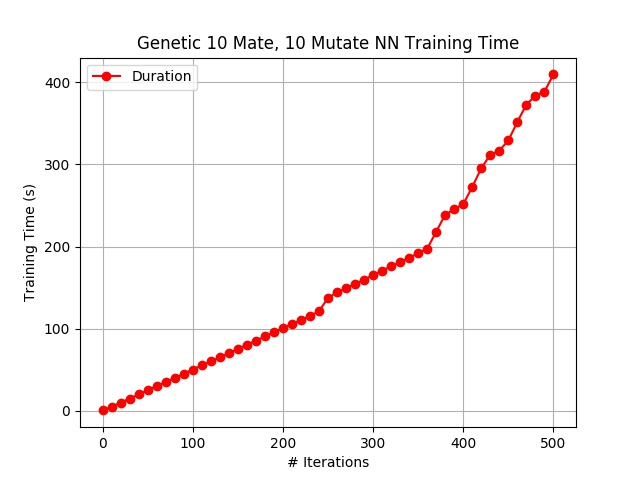
\includegraphics[width=1\textwidth,keepaspectratio]{genetic_10_mate,_10_mutate_nn_time.jpg} 
      \caption*{Genetic Algorithm Training Time w/ 10 Mate, 10 Mutate, 50 population} 
   \endminipage\hfill
   \minipage{0.49\textwidth}
      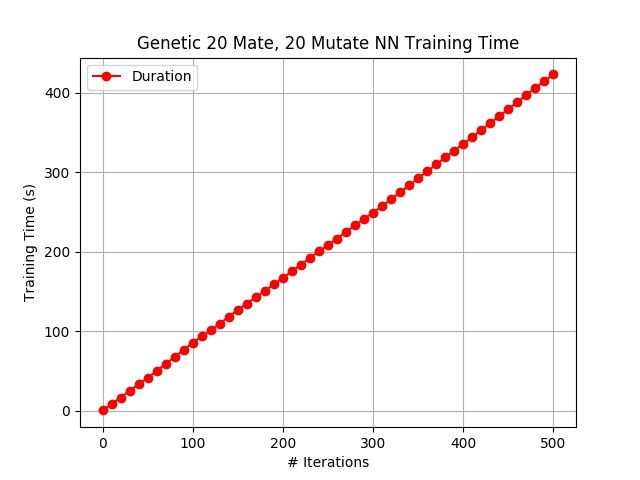
\includegraphics[width=1\textwidth,keepaspectratio]{genetic_20_mate,_20_mutate_nn_time.jpg} 
      \caption*{Genetic Algorithm Training Time w/ 20 Mate, 20 Mutate, 50 population} 
   \endminipage\hfill
\end{figure}


\subsection*{ Conclusion}  
The optimization algorithms used all inevitably produced similar results.  What 
differed, however, was the amount of training time required, the tuning of 
parameters, and how many iterations were required to achieve a consisent, 
optimal solution.  All-in-all, the genetic algorithm approach consistantly produced 
the best results for our network.  This makes sense, as the data was rather 
homogenous and there appeared to be very few outliers.  By learning the training 
data well, the learner was able to perform similarly well on the (nearly identical) 
test data.

\section*{Part 2: Optimization Problem Domains}
\subsection*{ Introduction}  
For this part of the assignment, three different optimization problems are 
examined: continous peaks, the traveling salesman, and flip flop.  The three
optimization techniques from above are used (randomized hill climbing, simulated annealing, and genetic algorithms) 
as well as another algorithm, MIMIC.
\\ \\
MIMIC, similar to the other algorithms, works to find the globally optimal 
solution.  Unlike the other algorithms, however, it retains knowledge of previous 
iterations and uses this information to more efficiently find better solutions.  MIMIC is particularly strong in regards to 
problems that maintain patterns between subsets of thier parameters.
\\ \\
Below, we apply each of the optimization algorithms to each of the three optimization 
problems.  We then look at how each optimization problem's characteristics may 
favor one algorithm to another, as well as evaluate the efficiency of each.

\subsection*{1) Continous Peaks}  
\subsubsection*{Overview}
The continous peaks problem is an extension of the four peaks problem that 
allows for a wide variety of local maximums.  This algorithm is particularly interesting due to the potentially large 
number of local maximums.  It is especially difficult for an algorithm that cannot escape 
local peaks to perform well.

 \begin{figure}[H]
  \minipage{0.32\textwidth}
      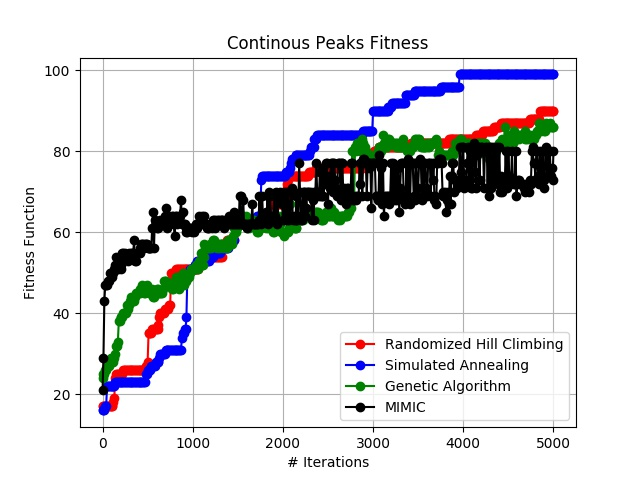
\includegraphics[width=1\textwidth,keepaspectratio]{continous_peaks_fitness.jpg} 
      \caption*{Fitness vs # Iterations of 4 Optimization Strategies} 
   \endminipage\hfill
   \minipage{0.32\textwidth}
      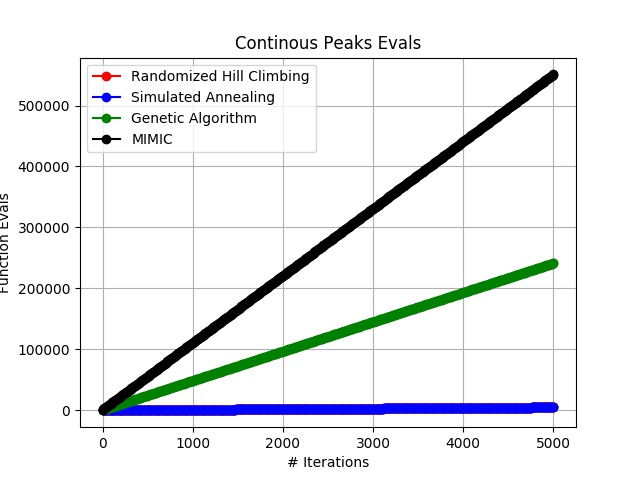
\includegraphics[width=1\textwidth,keepaspectratio]{continous_peaks_evals.jpg} 
      \caption*{Function Evals vs # Iterations of 4 Optimization Strategies} 
   \endminipage\hfill
   \minipage{0.32\textwidth}
      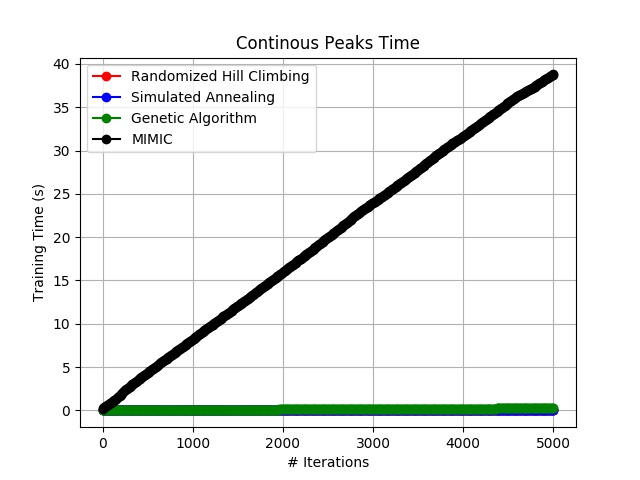
\includegraphics[width=1\textwidth,keepaspectratio]{continous_peaks_time.jpg} 
      \caption*{Training Time vs # Iterations of 4 Optimization Strategies} 
   \endminipage\hfill
\end{figure}

\subsubsection*{Analysis}

In order to ensure accuracy and a fair distribution, 5 different trials were 
used of 5000 iterations each.  Each optimization strategy was also allowed to evaluate over 
a parameter range in an attempt to find the optimal parameters for that 
strategy.
\\ \\
For randomized hill climbing, there were no other parameters to tune.  The 
algoritm was simply run for various iterations (multiples of 10) in a set of 5 
trials.  In terms of fitness function performance, it actually performed quite 
well and required no significant function evaluations. It was similarly fast to train due to the extreme simplicity 
of the algorithm itself. 
\\ \\
\begin{figure}[H] 
\begin{tabular}{ | c | c  | c | c | c | c | c |} 
\hline
\textbf{ } & \textbf{Fitness} & \textbf{Training Time} & \textbf{Function Evals}   \\
\hline
0 & 16.0 & 5.5038e-05 & 11 \\ \hline 
10 & 16.0 & 7.64649999999e-05 & 21 \\ \hline 
50 & 22.0 & 0.000212433 & 61 \\ \hline 
100 & 22.0 & 0.000370814 & 111 \\ \hline 
200 & 23.0 & 0.000717487 & 211 \\ \hline 
300 & 23.0 & 0.001094822 & 311 \\ \hline 
500 & 26.0 & 0.001666152 & 511 \\ \hline 
750 & 31.0 & 0.002682947 & 761 \\ \hline 
1000 & 51.0 & 0.003609291 & 1011 \\ \hline 
1500 & 62.0 & 0.005517988 & 1511 \\ \hline 
2000 & 74.0 & 0.007139624 & 2011 \\ \hline 
2500 & 84.0 & 0.008715217 & 2511 \\ \hline 
3000 & 90.0 & 0.010594833 & 3011 \\ \hline 
3500 & 95.0 & 0.012718942 & 3511 \\ \hline 
4000 & 99.0 & 0.014618306 & 4011 \\ \hline 
5000 & 99.0 & 0.018770859 & 5011 \\ \hline 

\end{tabular}
\caption*{Simulated Annealing Results w/ .15 Cooling} 
\end{figure}

Simulated annealing was slightly more complex, where cooling efficients of 0.15, 
0.35, 0.55, 0.75, and 0.95 were used.  It was found that the efficient 0.15 was 
the most effective here.  This low cooling rate was effective because it helped to slowly overcome any local
 maximums but not work too aggressively to skip any optimal solution.  By 
 iteration 3k, Simulated Annealing took a clear lead over the other solutions in 
 terms of fitness performance.  Similar to randomized hill climbing, its number 
 of function evals and training time was extremely low.
\\ \\
The genetic algorithm employed used a population size of 100 and various 
configurations of 50, 30, and 10 mutations/mate combinations.  The graph above 
depicts the succes rates when using 30 mutation and 30 matings.  As can be seen, 
it's performance was rather simular to randomized hill climbing--which roughly 
makes sense due to the random nature of both algorithms.  The number of function 
evaluations was higher for the genetic algorithm due to the amount of attempts 
at mutating and mating--whereas the training time was practically irrelevant.
\\ \\
Mimic's parameters were set to 100 samples and a 'to-keep' number of 50.  
The threshold for the discrete dependency tree mimic used was sampled from the 
range 0.1, 0.3, 0.5, 0.7, and 0.9.  While MIMIC started off relatively string in 
terms of fitness performance, it thrashed around the 60-80 range for the most 
part.  I had suspected that MIMIC would have difficulty on the continous peaks 
due to the large amount of randomness in the data.  The number of functional 
evaluations required for MIMIC was significnatly higher than the other 
algorithms, as was its training time.  This was primarily due to the fact that 
MIMIC is signifciantly more complex to operate than the other algorithms.
\\ \\
Overall, Simulated Annealing proved to be the best strategy for the continous 
peaks problem, largely due to it's ability to handle large amounts of randomness 
well and to avoid getting caught in such local maximums.  It's low training time 
and number of function evaluations further aided its case.


\subsection*{2) Traveling Salesman}  
\subsubsection*{Overview}
The traveling salesman problem is a frequently used, classic problem that focuses on a 
salesperson trying to minimize their round-trip distance between any number of cities.  This problem is particularly 
interesting  due to it's real-world implications, such as route planing for 
delivery trucks and everyday errands--it also has no known polynomial time 
solution!

 \begin{figure}[H]
  \minipage{0.32\textwidth}
      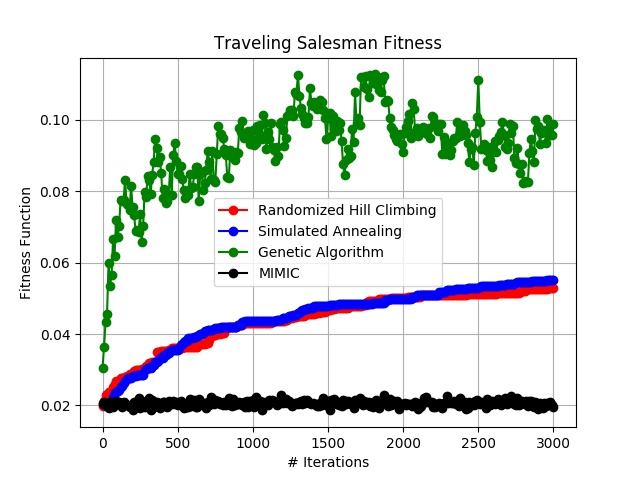
\includegraphics[width=1\textwidth,keepaspectratio]{traveling_salesman_fitness.jpg} 
      \caption*{Fitness vs # Iterations of 4 Optimization Strategies} 
   \endminipage\hfill
   \minipage{0.32\textwidth}
      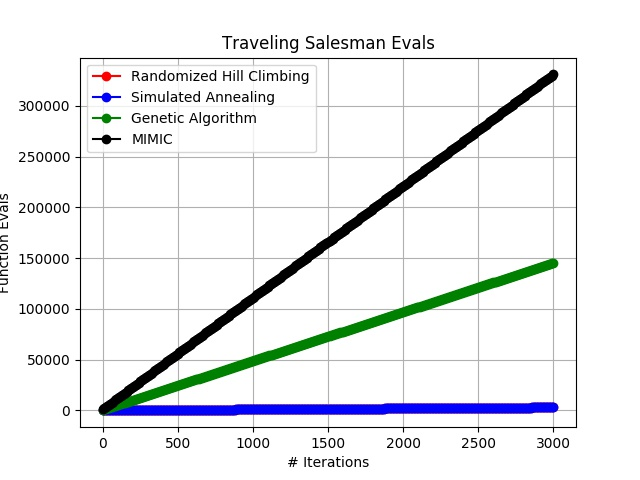
\includegraphics[width=1\textwidth,keepaspectratio]{traveling_salesman_evals.jpg} 
      \caption*{Function Evals vs # Iterations of 4 Optimization Strategies} 
   \endminipage\hfill
   \minipage{0.32\textwidth}
      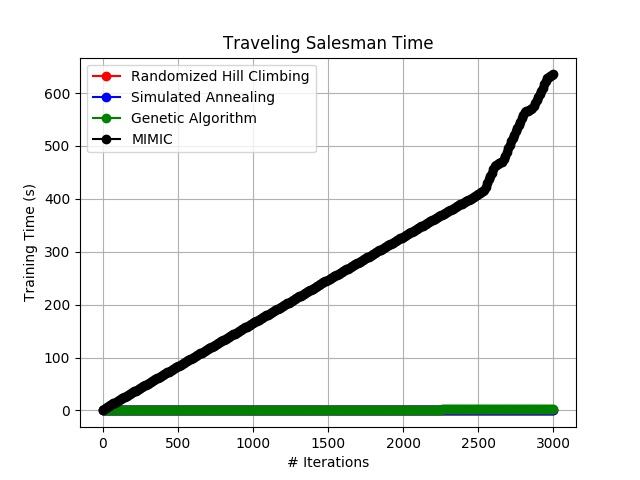
\includegraphics[width=1\textwidth,keepaspectratio]{traveling_salesman_time.jpg} 
      \caption*{Training Time vs # Iterations of 4 Optimization Strategies} 
   \endminipage\hfill
\end{figure}

\subsubsection*{Analysis}

For this optimization problem, in order to ensure accuracy and a fair distribution, 5 different trials were 
used of 3000 iterations each.  50 Random points were generated and used as the destinations for our faux salesman.
Each optimization strategy was also allowed to evaluate over 
a parameter range in an attempt to find the optimal parameters for that 
strategy.
\\ \\
For randomized hill climbing, there were no other parameters to tune.  The 
algoritm was simply run for various iterations in a set of 5 
trials.  In terms of fitness function performance, it performed mediocrely and required no significant function evaluations. It was similarly fast to train due to the extreme simplicity 
of the algorithm itself.  The reason for the stragegy's mediocrity can easily be 
attributed to the fact that random guessing does not perform well when trying to 
develop the most optimal path due to the large number of possibilities and low 
number of optimums.
\\ \\
Similar to the last problem, simulated annealing was slightly more complex, where cooling efficients of 0.15, 
0.35, 0.55, 0.75, and 0.95 were used.  It was found that the efficient 0.55 was 
the most effective here.  Interestingly enough, the simulated annealing approach very closely tracked the randomized hill climbing results. 
 This was pretty cool, and clearly demonstrated the effect of the problem on the 
 ability of a solution to perform well.  As both were prone to picking random 
 solutions and making marginal improvements on those solutions, they shared the 
 same strenghts and weaknesses for trying to plan an optimal path.  Similar to randomized hill climbing, simulated annealings' number 
 of function evals and training time was extremely low.
\\ \\
\begin{figure}[H] 
\begin{tabular}{ | c | c  | c | c | c | c | c |} 
\hline
\textbf{Iterations} & \textbf{Fitness} & \textbf{Training Time} & \textbf{Function Evals}   \\
\hline
0 & 0.0305500487733 & 0.011139866001 & 573 \\ \hline 
50 & 0.0535358597005 & 0.0619086620027 & 2984 \\ \hline 
100 & 0.0670653896105 & 0.106549986003 & 5404 \\ \hline 
200 & 0.0754973396223 & 0.190760427002 & 10194 \\ \hline 
300 & 0.0843530928911 & 0.276369227002 & 15021 \\ \hline 
500 & 0.0847430696768 & 0.430181398007 & 24690 \\ \hline 
750 & 0.0824751535861 & 0.62021527501 & 36716 \\ \hline 
1000 & 0.097111513149 & 0.799495104007 & 48778 \\ \hline 
1500 & 0.100315033444 & 1.153653522 & 72921 \\ \hline 
2000 & 0.0908447200981 & 1.51476069201 & 97068 \\ \hline 
2500 & 0.111066212921 & 1.875438519 & 121202 \\ \hline 
3000 & 0.0986916191186 & 2.27946003001 & 145282 \\ \hline 
\end{tabular}
\caption*{Genetic Algorithm Results w/ population 100, 30 mutations, 30 matings} 
\end{figure}

The genetic algorithm employed used a population size of 100 and various 
configurations of 50, 30, and 10 mutations/mate combinations.  The graph above 
depicts the succes rates when using 30 mutation and 30 matings.  As can be seen, 
it's performance was exceeding better than the other algorithms.  The mutations and matings were able to successfully 
identify the most optimal paths and plan extremelly well for the hypothetical salesman.  This can be attributed to 
the fact that traveling salesman can be broken into various subjourneys that the 
genetic algorithm can learn and then attempt to combine for an optimal journey.  The number of function  evaluations was higher for the genetic algorithm due to the amount of attempts 
at mutating and mating--whereas the training time was practically irrelevant.  
The genetic algorithm was the clear winner in terms of performance for the TSP.
\\ \\
Mimic's parameters were set to 100 samples and a 'to-keep' number of 50.  
The threshold for the discrete dependency tree mimic used was sampled from the 
range 0.1, 0.3, 0.5, 0.7, and 0.9.  MIMIC performed rather poorly on this problem.  This was very likely due to the fact that pattern finding is of almost no use in this 
problem domain and that previous knowledge also is mostly unnecessary when trying to find optimal paths.  The number of functional 
evaluations required for MIMIC was also significnatly higher than the other 
algorithms, as was its training time.  This was primarily due to the fact that 
MIMIC is signifciantly more complex to operate than the other algorithms.  
Overall, MIMIC was a very poor candidate for the traveling salesman problem.
\\ \\
Overall, the genetic algorithm proved to be the best strategy for the traveling salesman problem.  It's ability to combine 
sub-journeys and paths into an optimal route was strongly advantageous.  The results showed the strong benefit of mutations on this 
problem.  Similarly, it's speed an relative simplicity were also very 
beneficial.

\subsection*{3) Flip flop}  
\subsubsection*{Overview}
The flipflop problem is another common optimization, where one attempts to 
count the number of bits that alternate with its next neighbor in a bit string.  
This problem is particularly interesting because, since the strings are 
randomized, there is significant potential for a large number of local mimimum 
and maximums.  It is also particularly well suited for algorithms that can 
handle pattern matching  and previous knowledge well.  
\\ \\

 \begin{figure}[H]
  \minipage{0.32\textwidth}
      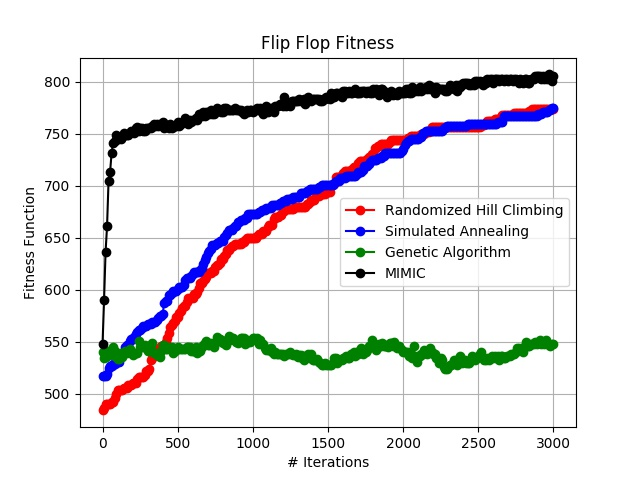
\includegraphics[width=1\textwidth,keepaspectratio]{flip_flop_fitness.jpg} 
      \caption*{Fitness vs # Iterations of 4 Optimization Strategies} 
   \endminipage\hfill
   \minipage{0.32\textwidth}
      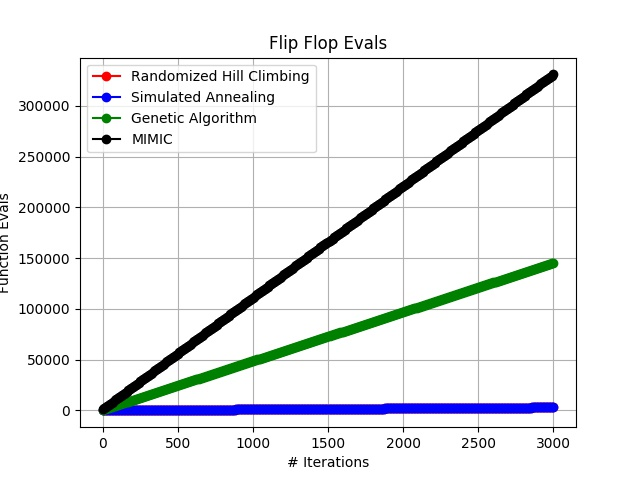
\includegraphics[width=1\textwidth,keepaspectratio]{flip_flop_evals.jpg} 
      \caption*{Function Evals vs # Iterations of 4 Optimization Strategies} 
   \endminipage\hfill
   \minipage{0.32\textwidth}
      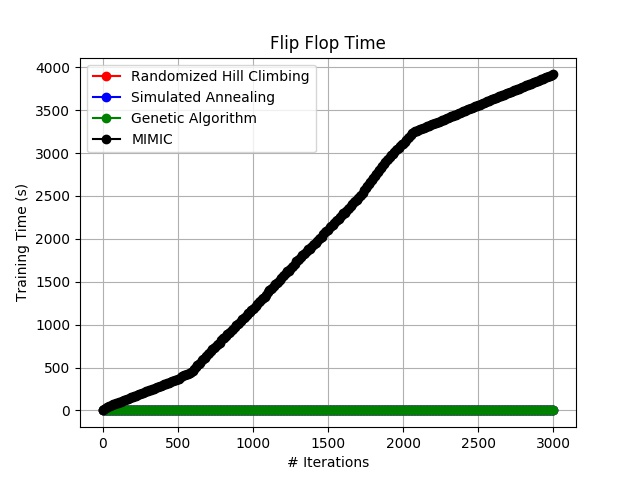
\includegraphics[width=1\textwidth,keepaspectratio]{flip_flop_time.jpg} 
      \caption*{Training Time vs # Iterations of 4 Optimization Strategies} 
   \endminipage\hfill
\end{figure}

\subsubsection*{Analysis}
For this optimization problem, in order to ensure accuracy and a fair distribution, 5 different trials were 
used of 3000 iterations each.  A bit string of length 1000 was used, where each 
bit was randomized as either 1 or 0.  Each optimization strategy was allowed to evaluate over 
a parameter range in an attempt to find the optimal parameters for that 
strategy.  The results are then summarized below.
\\ \\
For randomized hill climbing, there were no other parameters to tune.  The 
algoritm was simply run for various iterations in a set of 5 
trials.  In terms of fitness function performance, it actually performed rather well--with it's performance increasing over time. Randomized 
hill climbing required very limited function evaluations and it trained quickly due to its simplicity.  The reason for the stragegy's success can  be 
attributed to the fact that random guessing is somewhat akin to the distribution 
of the input bit string in that the distribution fo the next neighbor should, on 
average, change.
\\ \\
Similar to the last problem, simulated annealing was very similar to randomized hill climbing.  Cooling efficients of 0.15, 
0.35, 0.55, 0.75, and 0.95 were used.  It was found that the efficient 0.15 was 
the most effective in this case.  Simulated annealing approach closely tracked the randomized hill climbing results yet again. 
 Similar to hill climbing, the random variations of simulated annealing can roughly identify to the variations of the distribution of the input.  Over time, as with 
 randomized hill climbing, the performance of the strategy signficantly increased.  Also Similar to randomized hill climbing, its' 
 function evals count and training time were extremely low.
\\ \\

The genetic algorithm employed used a population size of 100 and various 
configurations of 50, 30, and 10 mutations/mate combinations.  The graph above 
depicts the succes rates when using 30 mutation and 30 matings.  The approach performed singificantly worse than the others.
  The genetic algorithm had a very tough time recognizing the pattern that the 
  input tended to follow and the mutations and matings had very little effect on 
  finding an optimal solution.  While t number of  evals was higher for the this strategy due to the amount of attempts 
at mutating and mating--it did not help to achieve a better result.
\\ \\

\begin{figure}[H] 
\begin{tabular}{ | c | c  | c | c | c | c | c |} 
\hline
\textbf{Iterations} & \textbf{Fitness} & \textbf{Training Time} & \textbf{Function Evals}   \\
\hline
0 & 548.0 & 10.292430561 & 1000 \\ \hline 
50 & 713.0 & 54.323489845 & 6500 \\ \hline 
100 & 745.0 & 89.781651075 & 12000  \\ \hline 
200 & 753.0 & 159.161412402 & 23000  \\ \hline 
300 & 755.0 & 227.402023603 & 34000  \\ \hline 
500 & 761.0 & 364.872433042 & 56000 \\ \hline 
750 & 771.0 & 741.847804258 & 83500 \\ \hline 
1000 & 771.0 & 1186.13889593 & 111000 \\ \hline 
1500 & 785.0 & 2107.83467502 & 166000 \\ \hline 
2000 & 789.0 & 3107.1784734 & 221000 \\ \hline 
2500 & 799.0 & 3557.31754274 & 276000 \\ \hline 
3000 & 805.0 & 3916.14983514 & 331000 \\ \hline 
\end{tabular}
\caption*{MIMIC Results w/ .5 threshold} 
\end{figure}

Mimic's parameters were set to 100 samples and a 'to-keep' number of 50.  
The threshold for the discrete dependency tree mimic used was sampled from the 
range 0.1, 0.3, 0.5, 0.7, and 0.9.  MIMIC performed incredbly on this problem--mainly due to its ability to handle patterns very well and to keep track of historical 
knowledge.  The number of 
evaluations required for MIMIC was definitely higher than the other 
algorithms, as was its training time, but its performance also far outweighed the other strategies.  
Overall, MIMIC proved incredibly succesful at the flip flop problem.

\subsection*{ Conclusion}  
Above, four different machine learning optimization strategies were applied to 3 
different optimization problems.  Interestingly enough, each optimization 
problem had its own inherit properties that proved more suitable for solving for 
differnet optimization strategies. 
\\ \\
The continous peaks problem, with its high amount of randomness and lack of 
predictable behaviour, proved to be optimized exceptionally well by simulated 
annealing.  Simulated annealings ability to randomly sample nearby solutions 
with effective cooling thresholds were very helpful for this problem in that it avoided getting trapped in local 
optimums but reduced the change of skipping over more significant nearby optimums.
\\ \\
The traveling salesman problem, which, in my opinion, proved to be the most 
interesting, was most aptly solved by a genetic algorithm.  Travelling salesman 
required various subjourneys to be optimized and combined to find an optimal 
path about various points.  Whereas random and pattern solutions failed badly, 
the genetic algorithm was able to mutate and combine to form optimal solutions 
quite well.
\\ \\
The final problem, flip flop, had an input that was highly repetetive and tended to follow 
a patterned distribution.  In such, optimization strategies that sought to solve 
based on subgroups of parameters or previous knowledge performed rather well, 
whereas strategies that were left to chance or random combinations performed 
poorly.  MIMIC, with it's ability to solve patterns and repetition well, as well 
as its ability to retain prior experiences, proved to be far and away the most optimal solution for this problem. 

\end{document}